\newpage
\section{Programming exercise : Applying decision trees and k-nearest neighbors \problemworth{50}}

\ifsoln
\else

\section*{Introduction\footnote{This assignment is adapted from the UCI Machine learning repository, available at \url{https://archive.ics.uci.edu/ml/datasets/adult}.}}

This data was extracted from the 1994 Census bureau database by Ronny Kohavi and Barry Becker. For computational reasons, we have already extracted a relatively clean subset of the data for this HW. The prediction task is to determine whether a person makes over \$50K a year.

In this problem, we ask you to complete the analysis of what sorts of people were likely to earn more than \$50K a year. In particular, we ask you to apply the tools of machine learning to predict which individuals are more likely to have high income. 


\section*{Starter Files}

\vspace{-\baselineskip}
\rule{\textwidth}{1pt}
code and data
\begin{itemize}[nolistsep]
    \item Code: \href{https://drive.google.com/file/d/10CFm6dfRr3WXjERC6sE682xVZhaewCPj/view?usp=share_link}{CS146-Winter2023-PS1.ipynb}\item Data: \href{https://drive.google.com/drive/folders/1bD0QyIc5Vum7g3kNpQ8yPz6EDPuzfasN?usp=sharing}{nutil.py and adult\_subsample.csv} 


\end{itemize}
documentation
\begin{itemize}[nolistsep]
\item Decision Tree Classifier: \\{\footnotesize \url{http://scikit-learn.org/stable/modules/generated/sklearn.tree.DecisionTreeClassifier.html}}
\item K-Nearest Neighbor Classifier: \\{\footnotesize \url{http://scikit-learn.org/stable/modules/generated/sklearn.neighbors.KNeighborsClassifier.html}} 
\item Cross-Validation: \\{\footnotesize \url{https://scikit-learn.org/stable/modules/generated/sklearn.model_selection.StratifiedShuffleSplit.html}}
\item Metrics: \\ {\footnotesize \url{http://scikit-learn.org/stable/modules/generated/sklearn.metrics.accuracy_score.html}, \\
\url{https://scikit-learn.org/stable/modules/generated/sklearn.metrics.f1_score.html?highlight=f1%20score#sklearn.metrics.f1_score}} 
\item Data Preprocessing: \\{\footnotesize \url{https://scikit-learn.org/stable/modules/generated/sklearn.preprocessing.StandardScaler.html?highlight=standardscaler#sklearn.preprocessing.StandardScaler}}
\end{itemize}
\vspace{-\baselineskip}
\rule{\textwidth}{1pt}


Note that any portions of the code that you must modify have been indicated with \verb|TODO|. Do not change any code outside of these blocks.
\fi

To work on this HW: you need to download two files (i) nutil.py (ii) adult\_subsample.csv from  \href{https://drive.google.com/drive/folders/1bD0QyIc5Vum7g3kNpQ8yPz6EDPuzfasN?usp=sharing}{here}. Then copy/upload them to you own Google drive. 

\ifsoln
\else
\clearpage
\fi

Next, for all the coding, please refer to the following colab notebook  
\href{https://drive.google.com/file/d/10CFm6dfRr3WXjERC6sE682xVZhaewCPj/view?usp=share_link}{CS146-Winter2023-PS1.ipynb}. 

\textbf{Before executing or writing down any code, please make a copy of the notebook and save it to your own google drive by clicking the File $\rightarrow$ Save a copy in Drive} 

\begin{minipage}[c]{.5\textwidth}
%\begin{figure}[H]
\centering
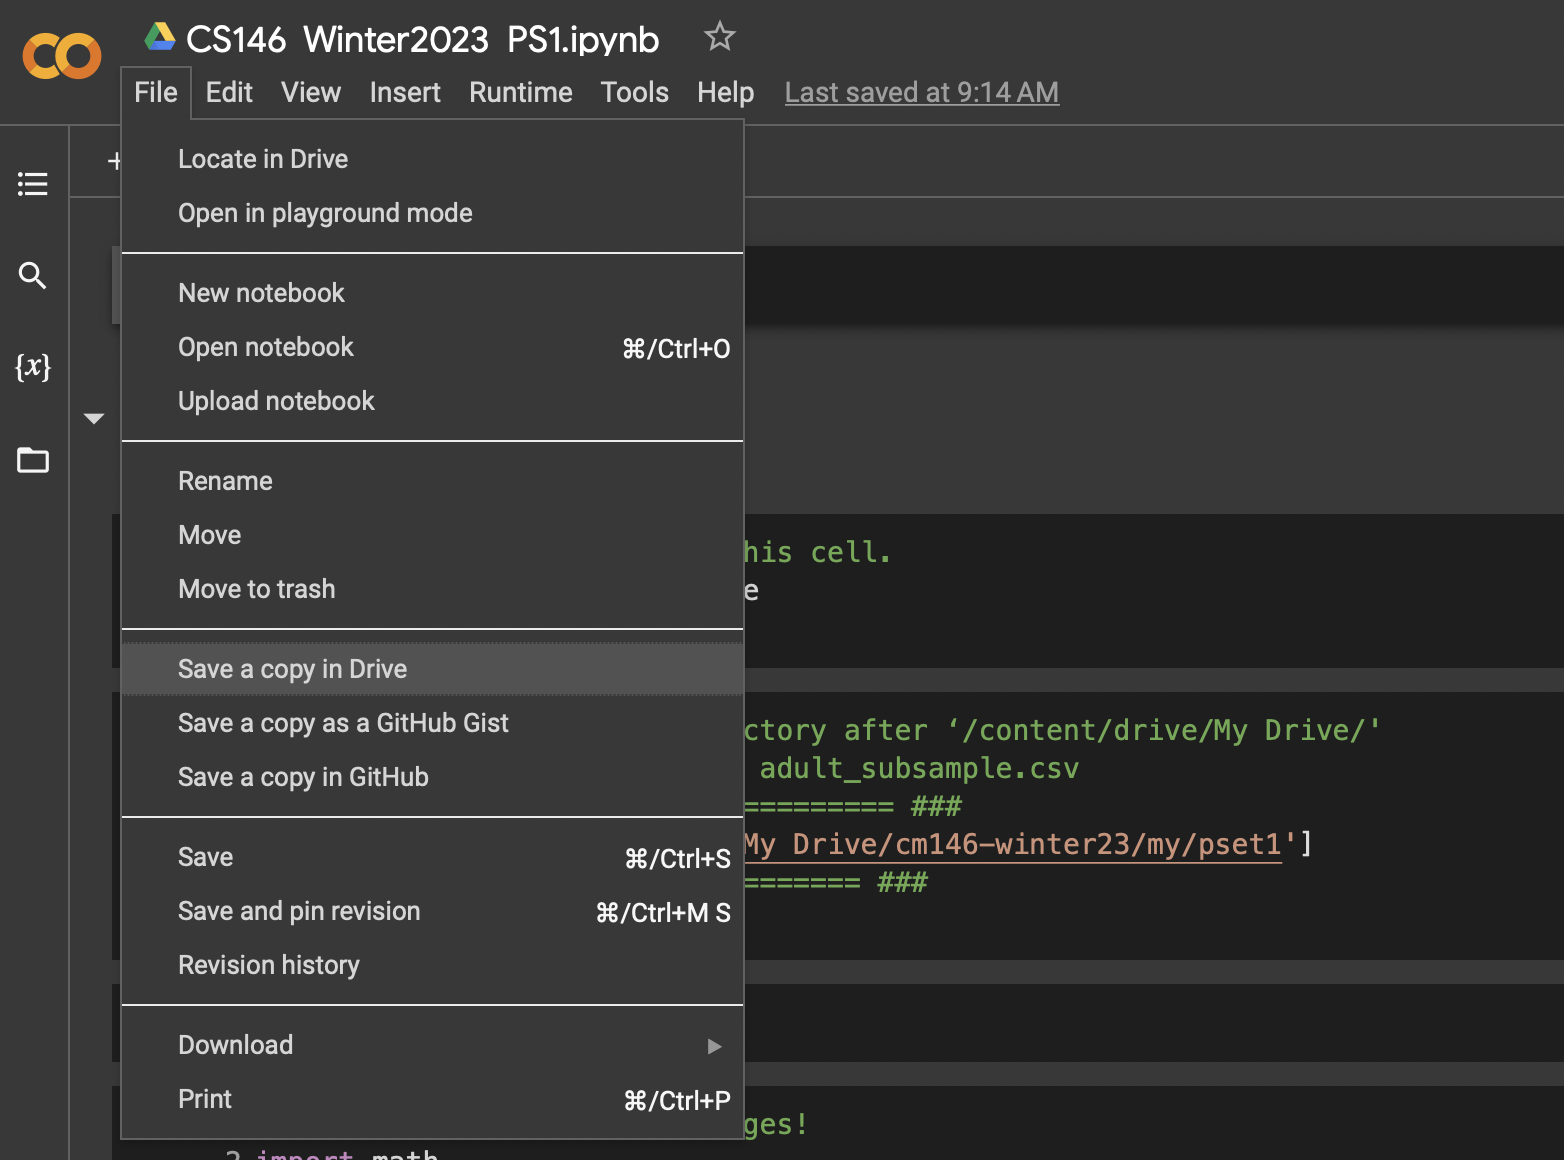
\includegraphics[scale=0.5]{save-colab-to-drive.png}
%\end{figure}
\end{minipage}%
\begin{minipage}[c]{.45\textwidth}
\end{minipage}%


You will then be prompted to log into your google account. Please make sure all the work you implement is done on your own saved copy. You won't to able to make changes on the the original notebook shared for the entire class. Running the first two cells will further mount your own google drive so that your copy of the Colab notebook will have access to the two files (nutil.py and adult\_subsample.csv) you have just uploaded.

The notebook has marked blocks where you need to code. \\
\\
 $\#\#\# ========= TODO  : START ========= \#\#\# $
 
 $\#\#\# ========= TODO :  END   ========== \#\#\#$
\\

\ifsoln
\else
\clearpage
\fi

\ifsoln
\else
\section*{Submission instructions}
\begin{itemize}
\item Only provide answers and plots through gradescope. Do not submit code.
\end{itemize}
\fi

For the questions please read below.

\subsection{Visualization \problemworth{5}}
One of the first things to do before trying any formal machine learning technique is to dive into the data. This can include looking for funny values in the data, looking for outliers, looking at the range of feature values, what features seem important, etc.

Note: We have already converted all the categorical features to numerical ones. The target column is the last one: "$>$50k", where 1 and 0 indicate $>$50k or $\le$ 50k respectively. The feature "fnlwgt" describes the number of people the census believes the entry represents. All the other feature names should be self-explanatory. If you want to learn more about this data please click  \href{https://archive.ics.uci.edu/ml/datasets/adult}{here}

\begin{enumerate}
\item \itemworth{5} Make histograms for each feature, separating the examples by class by running the function plot\_histograms in the notebook. This should produce fourteen plots, one for each feature, and each plot should have two overlapping histograms, with the color of the histogram indicating the class. For each feature, what trends do you observe in the data if any? (Please only describe the general trend. No need for more than two sentences per feature) 

\sol x

\begin{center}
    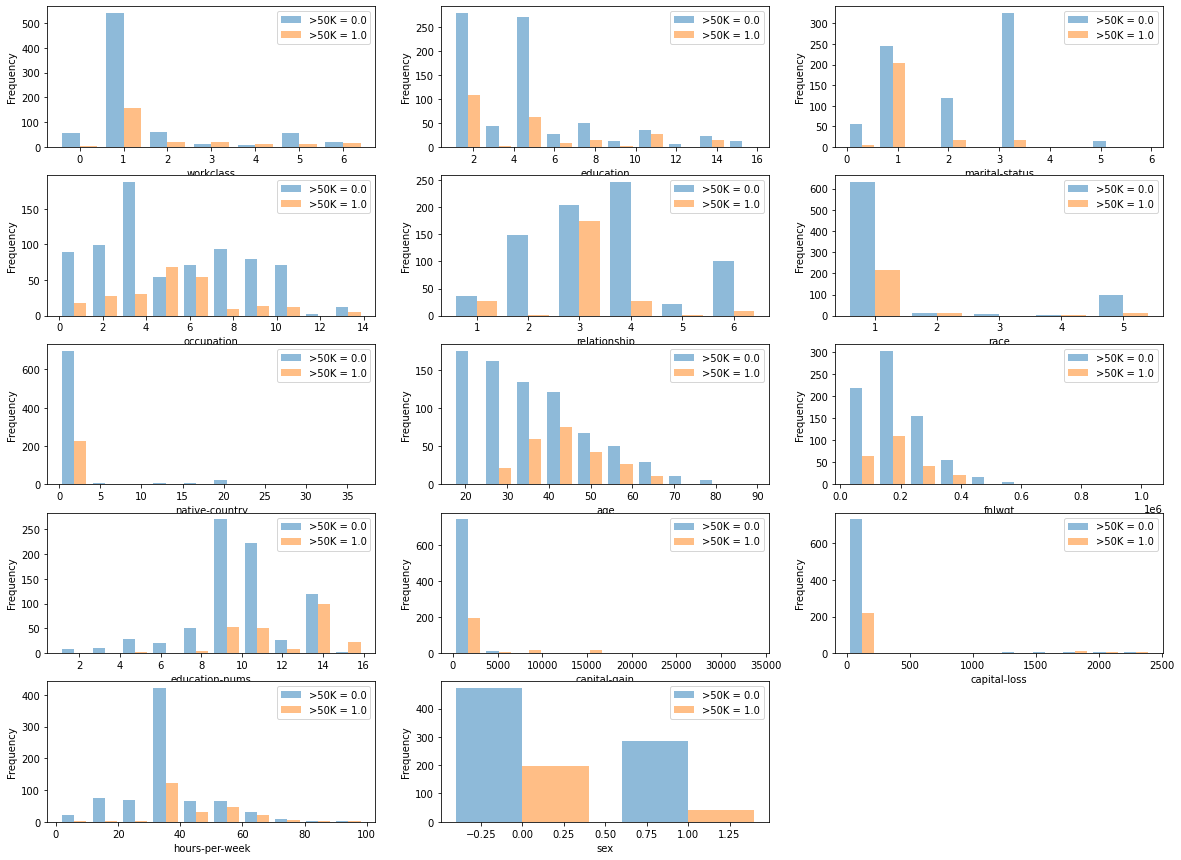
\includegraphics[scale=0.36]{5a.png} \\
\end{center}

The following analysis is conducted keeping in the mind the data markers from the linked resource:

\begin{itemize}
  \item Workclass: Most people are self-employed. Government workers are most likely to make $>$50k.
  \item Education: The more educated a person is, the more likely they are to make $>$50k.
  \item Marital Status: Divorced people are the most likely to make $>$50k.
  \item Occupation: Sales and exec-managerial are most likely to make $>$50k.
  \item Relationship: Husbands are more likely to make $>$50k.
  \item Race: Most people in this dataset are white, but Asians have a high fraction of people making $>$50k.
  \item Native Country: Most people in this study are from the USA. Most of these people make $<$50k.
  \item Age: People in the 40-50 age group are most likely to make $>$50k.
  \item Fnlwgt: The fraction of people making $>$50k is relatively constant. There are more people who make $<$50k.
  \item Education Nums: Most people have 8-10 years of education. People with >14 years of education have higher chances of making $>$50k.
  \item Capital Gain: Most people have a low capital gain. People with high capital gain tend to make $>$50k.
  \item Capital Loss: Most people have a low capital loss. People with high capital loss are evenly spread above the below the 50k mark.
  \item Hours per week: Most people work around 40 hours weekly. People who work more tend to earn $>$50k.
  \item Sex: There are more women in this study. Women have a higher chance of making $>$50k.
\end{itemize}

\end{enumerate}

\ifsolution{\newpage}
\subsection{Evaluation \problemworth{45}}

Now, let's use \verb|scikit-learn| to train a \verb|DecisionTreeClassifier| and \verb|KNeighborsClassifier| on the data.

Using the predictive capabilities of the \verb|scikit-learn| package is very simple. In fact, it can be carried out in three simple steps: initializing the model, fitting it to the training data, and predicting new values.\footnote{Note that almost all of the model techniques in \verb|scikit-learn| share a few common named functions, once they are initialized. You can always find out more about them in the documentation for each model. These are \verb|some-model-name.fit(...)|, \verb|some-model-name.predict(...)|, and \verb|some-model-name.score(...)|.}


\begin{enumerate}[resume]

\item \itemworth{0} Before trying out any classifier, it is often useful to establish a \emph{baseline}. We have implemented one simple baseline classifier, \verb|MajorityVoteClassifier|, that always predicts the majority class from the training set. Read through the \verb|MajorityVoteClassifier| and its usage and make sure you understand how it works.

Your goal is to implement and evaluate another baseline classifier, \verb|RandomClassifier|, that predicts a target class according to the distribution of classes in the training data set. For example, if 85\% of the examples in the training set have \verb|>50k = 0| and 15\% have \verb|>50k = 1|, then, when applied to a test set, \verb|RandomClassifier| should randomly predict 85\% of the examples as \verb|>50k = 0| and 15\% as \verb|>50k = 1|.

Implement the missing portions of \verb|RandomClassifier| according to the provided specifications. Then train your \verb|RandomClassifier| on the entire training data set, and evaluate its training error. If you implemented everything correctly, you should have an error of {\color {red} {$0.374$} } or {\color {red} {$0.385$.} }

\sol x Classifying using Random, training error: 0.374.

\item \itemworth{10} Now that we have a baseline, train and evaluate a \verb|DecisionTreeClassifier| (using the class from \verb|scikit-learn| and referring to the documentation as needed). Make sure you initialize your classifier with the appropriate parameters; in particular, use the `entropy' criterion discussed in class. What is the training error of this classifier?

\sol x Classifying using Decision Tree, training error: 0.000.

\item \itemworth{5} Similar to the previous question, train and evaluate a \verb|KNeighborsClassifier| (using the class from \verb|scikit-learn| and referring to the documentation as needed). Use $k$=3, 5 and 7 as the number of neighbors and report the training error of this classifier.

\sol x 

Classifying using k-Nearest Neighbors, training error for k = 3: 0.153; k = 5: 0.195; and k = 7: 0.213.

\item \itemworth{10} So far, we have looked only at training error, but as we learned in class, training error is a poor metric for evaluating classifiers. Let's use cross-validation instead.

Implement the missing portions of \verb|error(...)| according to the provided specifications. You may find it helpful to use \verb|StratifiedShuffleSplit(...)| from \verb|scikit-learn|. To ensure that we always get the same splits across different runs (and thus can compare the classifier results), set the \verb|random_state| parameter to be the same (e.g., 0).


Next, use your \verb|error(...)| function to evaluate the average cross-validation training error, test error and test micro averaged F1 Score (If you don\'t know what is F1, please click \href{https://scikit-learn.org/stable/modules/generated/sklearn.metrics.f1_score.html?highlight=f1\%20score#sklearn.metrics.f1_score}{here}) of each of your four models (for the \verb|KNeighborsClassifier|, use $k$=5). To do this, generate a random $80/20$ split of the training data, train each model on the $80\%$ fraction, evaluate the error on either the $80\%$ or the $20\%$ fraction, and repeat this $100$ times to get an average result. What are the average training and test error of each of your classifiers on the adult\_subsample data set?

\sol x 

Investigating various classifiers:

Majority: Train error = 0.240, Test error = 0.240, F1 score: 0.760; \\
Random: Train error = 0.375, Test error = 0.382, F1 score: 0.618; \\
Decision Tree: Train error = 0.000, Test error = 0.205, F1 score: 0.795; \\
KNN: Train error = 0.202, Test error = 0.259, F1 score: 0.741.

\item \itemworth{5} One way to find out the best value of $k$ for \verb|KNeighborsClassifier| is $n$-fold cross validation.
Find out the best value of $k$ using 10-fold cross validation. You may find the \verb|cross_val_score(...)| from \verb|scikit-learn| helpful. Run 10-fold cross validation for all odd numbers ranging from 1 to 50 as the number of neighbors.
Then plot the validation error against the number of neighbors, $k$.
Include this plot in your writeup, and provide a 1-2 sentence description of your observations. What is the best value of $k$?

\sol x

\begin{center}
    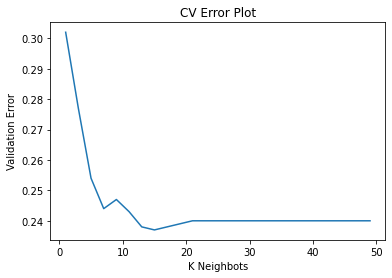
\includegraphics[scale=0.6]{5f.png} \\
\end{center}

As k increases, the validation error decreases until k = 21, post which the error stagnates. The best value of k is 15, with an error value of 0.237.

\item \itemworth{5} One problem with decision trees is that they can \emph{overfit} to training data, yielding complex classifiers that do not generalize well to new data. Let's see whether this is the case.

One way to prevent decision trees from overfitting is to limit their depth. Repeat your cross-validation experiments but for increasing depth limits, specifically, $1,2,\ldots,20$. You may find \verb|cross_validate(...)| from \verb|scikit-learn| helpful. Then plot the average training error and test error against the depth limit. 
Include this plot in your writeup, making sure to label all axes and include a legend for your classifiers. What is the best depth limit to use for this data? Do you see overfitting? Justify your answers using the plot.

\sol x 

\begin{center}
    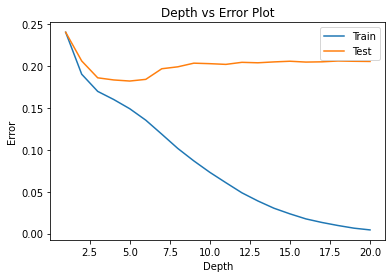
\includegraphics[scale=0.6]{5g.png} \\
\end{center}

The best depth limit for this data is 5.0, with a testing error of 0.181. Overfitting is observable in the graph after a depth of 5.0. This is because the testing error increases in that range.

\item \itemworth{5} Another useful tool for evaluating classifiers is \emph{learning curves}, which show how classifier performance (e.g. error) relates to experience (e.g. amount of training data).
For this experiment, first generate a random 90/10 split of the training data using \verb|train_test_split| from \verb|scikit-learn| with \verb|random_state| set to 0. Then, do the following experiments considering the 90\% fraction as training and 10\% for testing. 

Run experiments for the decision tree and k-nearest neighbors classifier with the best depth limit and $k$ value you found above.
This time, vary the amount of training data by starting with splits of $0.10$ ($10\%$ of the data from 90\% fraction) and working up to full size $1.00$ ($100\%$ of the data from 90\% fraction) in increments of $0.10$. Then plot the decision tree and k-nearest neighbors training and test error against the amount of training data. 
Include this plot in your writeup, and provide a 1-2 sentence description of your observations.

\sol x 

\begin{center}
    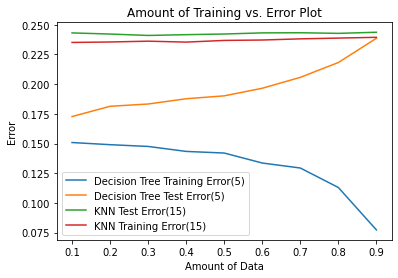
\includegraphics[scale=0.6]{5h.png} \\
\end{center}

The Decision Tree error increases with the amount of training data. The training error is always less than the testing error.

\item \itemworth{5} Pre-process the data by standardizing it. See the sklearn.preprocessing.StandardScaler package for details. After performing the standardization such as normalization please run all previous steps part (b) to part (h) and report what difference you see in performance.   \\

\sol x

\begin{center}
    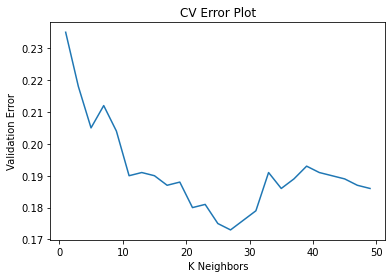
\includegraphics[scale=0.6]{5i-1.png} \\
    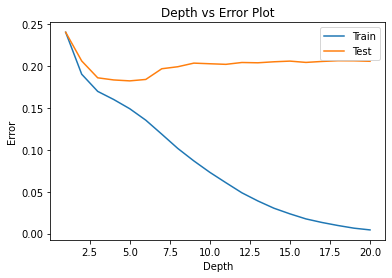
\includegraphics[scale=0.6]{5i-2.png} \\
    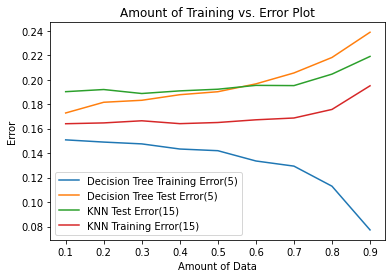
\includegraphics[scale=0.6]{5i-3.png} \\
\end{center}

Classifying using Majority Vote, training error: 0.240.

Classifying using Random, training error: 0.374.

Classifying using Decision Tree, training error: 0.000.

Classifying using k-Nearest Neighbors, training error for k = 3: 0.114; k = 5: 0.129; and k = 7: 0.152.
 
Majority: Train error = 0.240, Test error = 0.240, F1 score: 0.760; \\
Random: Train error = 0.375, Test error = 0.382, F1 score: 0.618; \\
Decision Tree: Train error = 0.000, Test error = 0.205, F1 score: 0.795; \\
KNN: Train error = 0.133, Test error = 0.209, F1 score: 0.791.

Observations: For Random, Decision Tree, and Majority, the performance remains the same. KNN performance, however, significantly increases. Additionally, the best k value increases to 25-27.

\end{enumerate}


